\chapter[SCP-009 红冰]{
	SCP-009 Red Ice\\
	SCP-009 红冰
}

\label{chap:SCP-009}

\begin{figure}[H]
	\centering
	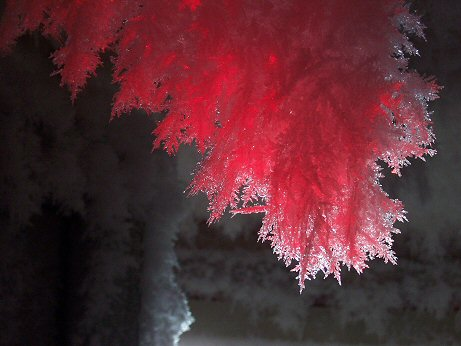
\includegraphics[width=0.5\linewidth]{images/SCP.009.jpg}
	\caption*{回收之前的SCP-009}
\end{figure}

\bb{项目编号:}SCP-009

\bb{项目等级:}Euclid

\bb{特殊收容措施:}对象需要被安置于 14 立方米以上的用隔热合金制作的密闭水槽中。

SCP-009在除了实验的任何情况下都不允许被暴露在0℃以上的环境中。在收容措施的30米内不允许存在任何常温状况下是液体的固态物(除了冰)。对象的收容设施中需要装有温度传感器并被一直监控,需要有不少于 3 台的制冷机保持制冷。任何温度传感器或制冷系统的故障需要被汇报并立即维修。

若收容措施中的温度上升到-5℃以上,收容措施需立即被封闭,并被制冷剂浸没直到温度下降到-25℃至-30℃之间。有人员进入时收容区必须保持真空,收容措施中的水蒸气需要被过滤并在与收容措施相同的环境下隔离24小时以上。任何展现出SCP-009特性的水蒸气需要被隔离并尽快加入收容措施中。

任何观察SCP-009或与之接触的人需要穿着环境防护服。离开收容措施的所有人员所携带的工具,研究材料和其它与SCP-009的收容措施有过接触的物品需要进行脱水处理。若发现污染物,任何人员或材料都不允许离开,并开始对收容区进行二级隔离。极端情况下可以处决目标,但安全卫队必须离目标尽可能远以确保不接触受SCP-009污染的液体。

\bb{描述:}SCP-009是大约 3700 公升(L)展现出很多奇异特性的物质。小部分物质,在所有时期,都与水相近,但大部分物质都呈现深红色。

无论如何,它最显著的特点是对温度变化的反应对普通H\textsubscript{2}O非常不同:对象在-100℃至0℃时是液体状态,在超过此温度时为固体状态,在-100℃以下蒸发为水蒸气一样的气体,但在高压下仍保持红色。

对对象进行的原子结构实验没有明确的结果。测试表明对象与普通的水一样由氢和氧组成,这不禁让研究人员推测,对象异常状况的根源在于其原子本身。██████博士则主张对象来源于一个物理法则颠倒的世界,或是被那个世界改变了性质。

这一推测在解释对象将普通的水“同化”至与它相同的显著能力时有一定的价值。若与液体(可以是冰,盐水,空气中的水蒸气)有任何物理接触,SCP-009就会“传播”并污染它,使它展现出对象的特性。尽管这一特性在任何状态下都有所展现,但这一进程在液体状态下是最慢(也是最可控)的。

若对象与任何生物的热源接触,生物的体液会迅速被SCP-009转化,因为生物体的体温,被转化的体液会很快冻结(哺乳动物因为它们的高体温更易受影响)。因为SCP-009冻结时会放热(与冰融化时放热速率相同),这一进程会持续直到所有可能的液体被转化或被外部干扰中止。

在D级人员上的实验表明了对象转化的过程,概括为以下几步:

1.最初接触:实验对象暴露于SCP-009,它表现出特性并开始转化接触面(通常为皮肤)上的任何水分。若存在薄雾,雾,雪或其它固态或液态的水则会大大的加剧这一过程。

2.表层转化:被转化的一薄层区域因为体温与SCP-009产生的热量在冻结中升高温度。这一过程可在任何部位发生,并根据实验对象的体温持续5分钟至1小时不等。在这一阶段,冻结的进程穿过了表皮并迅速到达活细胞。

3.深层转化:温度升高造成的冰的体积膨胀贯穿了受试者的身体,造成细胞从内部破裂。因为晶体溢满了伤口,现阶段基本不会流血,受测者可以继续存活并保持意识清醒██小时。

4.[数据删除]

5.死亡:身体内多个器官停止工作,血液循环因血液晶体化停止。

在D级人员上的实验自4/23/20██停止。

\bb{附录:对象被回收时的情况:}对象于11/05/19██在阿拉斯加的████被发现。基金会在接到了当地居民████ Tribe的报告后介入,他穿过了村庄██米外的一艘看似发生海难的捕杀海豹的船只上面的破碎的尸体。\\
所有受害者的尸体都被红色的冰包裹。死亡的原因被记录为为内出血。在完整的遗体上,观察到了受害者惊恐和剧痛的表情。据此推测较低的环境温度减缓了结冰的过程。这延长了转化时间至██小时,并使受害者保持意识清醒直到[数据删除]。

\bb{附录:}12/16/20██\\
在另行通知之前,禁止对009进行超低温实验。员工只能对可控量的对象使用液态氮,并只能在温度达到可接受的水平时。\\
相关说明:SCP-009在冷核聚变研究中可能的应用有待评估。
